\documentclass{beamer}
\usetheme{CambridgeUS}
\usepackage{tikz}
\usepackage{graphicx}

\title{Kubernetes CronJob Controller}
\author{avengeHERs}
\date{27th June 2024}
\begin{document}

\frame{\titlepage}
\begin{frame}
\frametitle{Here's the team!}

\begin{itemize}
    \item Meghna Mandawra
    \item Srishti Dutta
    \item Khushi S.
\end{itemize}

\end{frame}


\begin{frame}

\frametitle{Idea}

We aim to develop a custom Kubernetes CronJob controller using Go.
\begin{itemize}
    \item Objective: Develop a basic custom Kubernetes controller using Go.
    \item Purpose: Learn and understand the fundamentals of Kubernetes and its controller development.
\end{itemize}
\begin{figure}
    \centering
    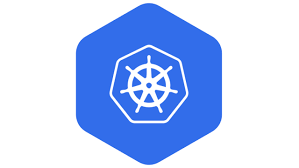
\includegraphics[width=0.5\textwidth]{k8simg.png}
    \caption{Kubernetes}
\end{figure}
\end{frame}

\begin{frame}
\frametitle{What is Kubernetes (K8s)?}
\begin{itemize}
    \item It is a container orchestration platform that helps in automating the deployment, scaling, and management of containerized applications.\par 
    \item Think of Kubernetes as a manager for your application containers, ensuring they run smoothly, are scaled correctly, and recover from failures.
\end{itemize}


    \begin{block}{}
      K8s: Deploy, Scale, Chill.
    \end{block}
    \begin{figure}
        \centering
        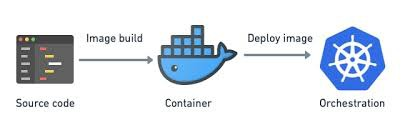
\includegraphics[width=0.5\textwidth]{whatisk8.jpg} 
    \end{figure} 
\end{frame}

\begin{frame}
\frametitle{Why K8s?}
\begin{itemize}
    \item<1->  Trend from Monolith to Microservices.\pause
    \item<2-> Increased usage of containers. \pause
    \item<3-> Demand for a proper way of managing those hundreds of containers.
\end{itemize}
\begin{figure}
    \centering
    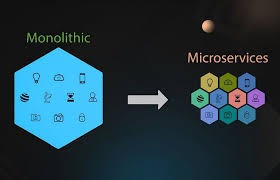
\includegraphics[width=0.5\textwidth]{whyk8.jpg}
\end{figure}
\end{frame}

\begin{frame}
\frametitle{Inside K8s : The role of Controllers}
\begin{itemize}
    \item Control loops that maintain the desired state of cluster resources.\pause
    \item Automate tasks like scaling, updates, and resource management.\pause
\end{itemize}
\begin{figure}
    \centering
    
\includegraphics[width=0.7\textwidth]{controllers.png}
\end{figure}

\end{frame}
\begin{frame}
\frametitle{The CronJob Controller}
A CronJob controller in Kubernetes is like a scheduler or a task manager for your applications running in a Kubernetes cluster.
It allows you to automate repetitive tasks that need to be performed at specific times or intervals.

\end{frame}
\begin{frame}
\frametitle{Tool Chain}
\begin{itemize}
\item Programming Language: Go (Golang)
\item Kubernetes Client Library: client-go
\item Controller Framework: controller-runtime
\item Development Tools: Go tools (go), go mod
\item Testing Framework: Go testing package, controller-runtime testing utilities
\item Containerization: Docker
\item KubeBuilder Framework
\item Version Control: Git
\end{itemize}
\end{frame}

\begin{frame}
    \frametitle{Plan of action}

    \begin{itemize}
        \item Learn Go
        \item Learn Kubernetes concepts 
        \item Environment Setup
        \item Design and Implementation 
        \begin{itemize}
            \item Design Custom Resource Definitions (CRDs)
            \item Develop CronJob Controller
            \item Integrate with Kubernetes API 
            \item Update the mentors regarding the progress after a week , take feedback and work accordingly.
        \end{itemize}
        \item Testing and Quality Assurance
        \item Deployment 
    \end{itemize}
\end{frame}
\begin{frame}
    \frametitle{Resources}

    \begin{itemize}
        \item Kubernetes Documentation - https://kubernetes.io/
        \item  Go Documentation - https://go.dev/doc/
        
    \end{itemize}
\end{frame}
\begin{frame}
    \frametitle{Thank you}
    fmt.Println("Thank you")
\end{frame}
    
\end{document}





